% Paper template for TAR 2022
% (C) 2014 Jan Šnajder, Goran Glavaš, Domagoj Alagić, Mladen Karan
% TakeLab, FER

\documentclass[10pt, a4paper]{article}

\usepackage{tar2023}

\usepackage[utf8]{inputenc}
\usepackage[pdftex]{graphicx}
\usepackage{booktabs}
\usepackage{amsmath}
\usepackage{amssymb}
\usepackage{cleveref}

\title{Stress Analysis in Social Media}

\name{Sven Šćekić, Marko Kuzmić, Lovro Bučar}

\address{
    University of Zagreb, Faculty of Electrical Engineering and Computing\\
    Unska 3, 10000 Zagreb, Croatia\\
    \texttt{\{sven.scekic, marko.kuzmic, lovro.bucar\}@fer.hr}\\
}


\abstract{
    Here we can write an abstract of the paper.
    The abstract is a paragraph of text ranging between 70 and 150 words.
}

\begin{document}

\maketitleabstract

\section{Introduction}

This section is the introduction to your paper.

\section{Related Work}

In scientific papers, this section usually ( but not necessarily ) briefly describes the related research and what makes the presented approach different from it.
Demonstration of citing~\citep{maguire-76}.

\section{Dataset}

A section that will be used to describe the dataset that was used in the research paper.

\section{Models}
Motivated by the results of the before mentioned paper, our approach focused on three different models which solve the given classification problem.
\hfill \break
\hfill \break
Firstly we will introduce the \textbf{logistic regression} model which the authors of the dataset presented as the best solution, excluding state-of-the-art solutions such as BERT.
Then we are going to introduce two transformer approaches, one being \textbf{DistilBERT} and the other one, currently very popular, \textbf{Chat GPT 3.5 Turbo}.

\subsection{Preprocessing}
Before we trained our models we needed to do some form of preprocessing on our data.
This step is important because it enables adequate learning from the training set.
Given the dataset already contained pretty clean and structured data, we didn't need to do a lot of preprocessing to get the desired results.
We started with the basic stop word removal, followed by digit and punctuation removal.
Then we performed lemmatization which enabled us to properly train the word embeddings for the logistic regression model and tokenizer for the DistilBERT model.

\subsection{Logistic regression}
Logistic regression is a commonly used machine learning model which can be used for binary classification problem.
This is a simple model which doesn't require long and expensive training, so, inspired by the great results that this model showed in the original paper (F-score of 79.8 ~\citep{turcan-mckeown-2019-dreaddit}), we have also decided to
include it in our own research.
\hfill \break
\hfill \break
Logistic regression model expects a fixed size input but words and sentences in natural language can be of any size.
Today this problem is solved by using word embeddings which represent words from our dataset as multidimensional vectors. Their advantage over some other approaches that were used in the past, such as one-hot vector representation, is that they are able to find relations between words and produce similar vectors for similar words.In our approach we used \textbf{word2Vec}~\citep{mikolov2013efficient} embeddings which were trained on the whole training dataset and produced 300-dimensional representations.
Learned word embeddings were then used for calculating the final representation for each training example.
Here we experimented with 2 approaches:
\begin{enumerate}
    \item \label{itm:one} \textbf{Averaging of word embeddings:} summing up each representation in the input sequence and dividing it with the number of words in the sequence
    \item \textbf{TF-IDF averaging:} Term Frequency - Inverse Document Frequency is an algorithm that is used to determine an importance of the given word in the document.
    Importance is represented as a scalar value.
     This scalar value for each word is then multiplied with the word's corresponding representation.
    The final representation is then calculated in the same way as described in~\ref{itm:one}.

\end{enumerate}

\subsection{DistilBERT}
The second model we used was DistilBERT~\citep{sanh2020distilbert}.
This model comes from the family of deep learning models called transformers~\citep{vaswani2017attention}.
The main advantage of these types of models is the self-attention mechanism.
Self-attention allows the model to find the importance of each word in a sequence and build more effective contextual representations.
\hfill \break
\hfill \break
DistilBERT is a model similar to the more popular BERT~\citep{devlin2019bert}, but faster and more lightweight while still preserving almost all the capabilities of the larger model.
Because of its features and our limited hardware we decided it would be the best option for representing current SOTA solution in the field of transformers.
Model and tokenizer were trained simultaneously on the whole training set using the implementations from the \textit{HuggingFace} library.


\subsection{Chat GPT 3.5 Turbo}

\begin{figure}
    \centering
    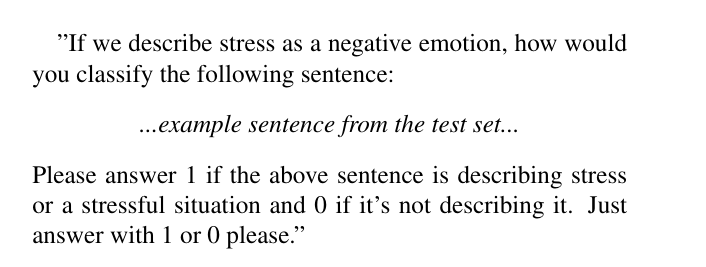
\includegraphics[width=0.5\textwidth]{images/chat-gpt-prompt}
    \caption{Text input for Chat GPT 3.5 Turbo API}
    \label{fig:chat-gpt-prompt}
\end{figure}

The final model that we used in our research was Chat GPT 3.5 Turbo.
This model was developed by OpenAI and it aims to generate human like responses based on the provided input text.
We couldn't perform direct training on this model, but instead we used the provided API to prompt the model to give us the classification result for each example in the test set.
You can see how we formulated our prompt in figure~\ref{fig:chat-gpt-prompt}.

Given results were then cleaned up

\section{Results}

Finally, a section which describes the acquired results.

\section{Conclusion}

Conclusion is the last enumerated section of the paper.
It should not exceed half of a column and is typically split into 2--3 paragraphs.
No new information should be presented in the conclusion; this section only summarizes and concludes the paper.

\section*{Acknowledgements}

Here we can write a thank you to the professors and the assistants which were involved in TAR class.

\bibliographystyle{tar2023}
\bibliography{tar2023}

\end{document}

